\documentclass[zavrsnirad]{fer}
% Dodaj opciju upload za generiranje konačne verzije koja se učitava na FERWeb
% Add the option upload to generate the final version which is uploaded to FERWeb


\usepackage{blindtext}
\usepackage{amssymb}


%--- PODACI O RADU / THESIS INFORMATION ----------------------------------------

% Naslov na engleskom jeziku / Title in English
\title{Demonstrative framework for differenciable programming}

% Naslov na hrvatskom jeziku / Title in Croatian
\naslov{Demonstracijski okvir za diferencijabilno programiranje}

% Broj rada / Thesis number
\brojrada{1665}

% Autor / Author
\author{Jakov Novak}

% Mentor 
\mentor{Prof. dr. sc. Siniša Šegvić}

% Datum rada na engleskom jeziku / Date in English
\date{June, 2024}

% Datum rada na hrvatskom jeziku / Date in Croatian
\datum{lipanj, 2024.}

%-------------------------------------------------------------------------------


\begin{document}


% Naslovnica se automatski generira / Titlepage is automatically generated
\maketitle


%--- ZADATAK / THESIS ASSIGNMENT -----------------------------------------------

% Zadatak se ubacuje iz vanjske datoteke / Thesis assignment is included from external file
% Upiši ime PDF datoteke preuzete s FERWeb-a / Enter the filename of the PDF downloaded from FERWeb
\zadatak{zadatak.pdf}


%--- ZAHVALE / ACKNOWLEDGMENT --------------------------------------------------

\begin{zahvale}
  % Ovdje upišite zahvale / Write in the acknowledgment
  Hvala na kavi...
\end{zahvale}


% Odovud započinje numeriranje stranica / Page numbering starts from here
\mainmatter


% Sadržaj se automatski generira / Table of contents is automatically generated
\tableofcontents


%--- UVOD / INTRODUCTION -------------------------------------------------------
\chapter{Uvod}
\label{pog:uvod}

\section{Motivacija}
Većina klasičnih postupaka u dubokom učenju se svode na optimizaciju izlaza neuralne mreže s obzirom na neku funkciju gubitka. Kod takvih postupaka je ključan izračun gradijenta te funkcije kako bi se podesile značajke mreže:
\begin{equation}
  \nabla (f \circ L) (ulaz)
\end{equation}
Postoje različiti pristupi u korištenju računala za rješavanje tog problema. Neki od glavnih su: simboličko diferenciranje, numeričke metode i automatska diferencijacija. Glavni nedostatci prvih spomenutih pristupa su prevelika složenost dobivenih izraza (citation needed) i nepreciznost brojeva s pomičnim zarezom (citation needed). Ovaj rad je fokusiran na proučavanju metoda automatske diferencijacije te implementacije jednostavnog demonstracijskog okvira u programskom jeziku C++ uz pomoć biblioteke OpenCL za matrične operacije.

\section{Metode automatske diferencijacije}
Glavna ideja automatske diferencijacije jest da dobivenu matematičku funkciju možemo prikazati kao aciklički digraf kojemu su čvorovi varijable, konstante ili međurezultati: $G = (V, E). V = Var \cup F$, gdje je $Var$ skup varijabli, a $F$ skup primitivnih funkcija koje se lako mogu derivirati. Ulaz neke funkcije $f \in F$ je definiran kao: $\{x \in V \colon (x, f) \in E\}$
\begin{figure}[h]
  \centering
  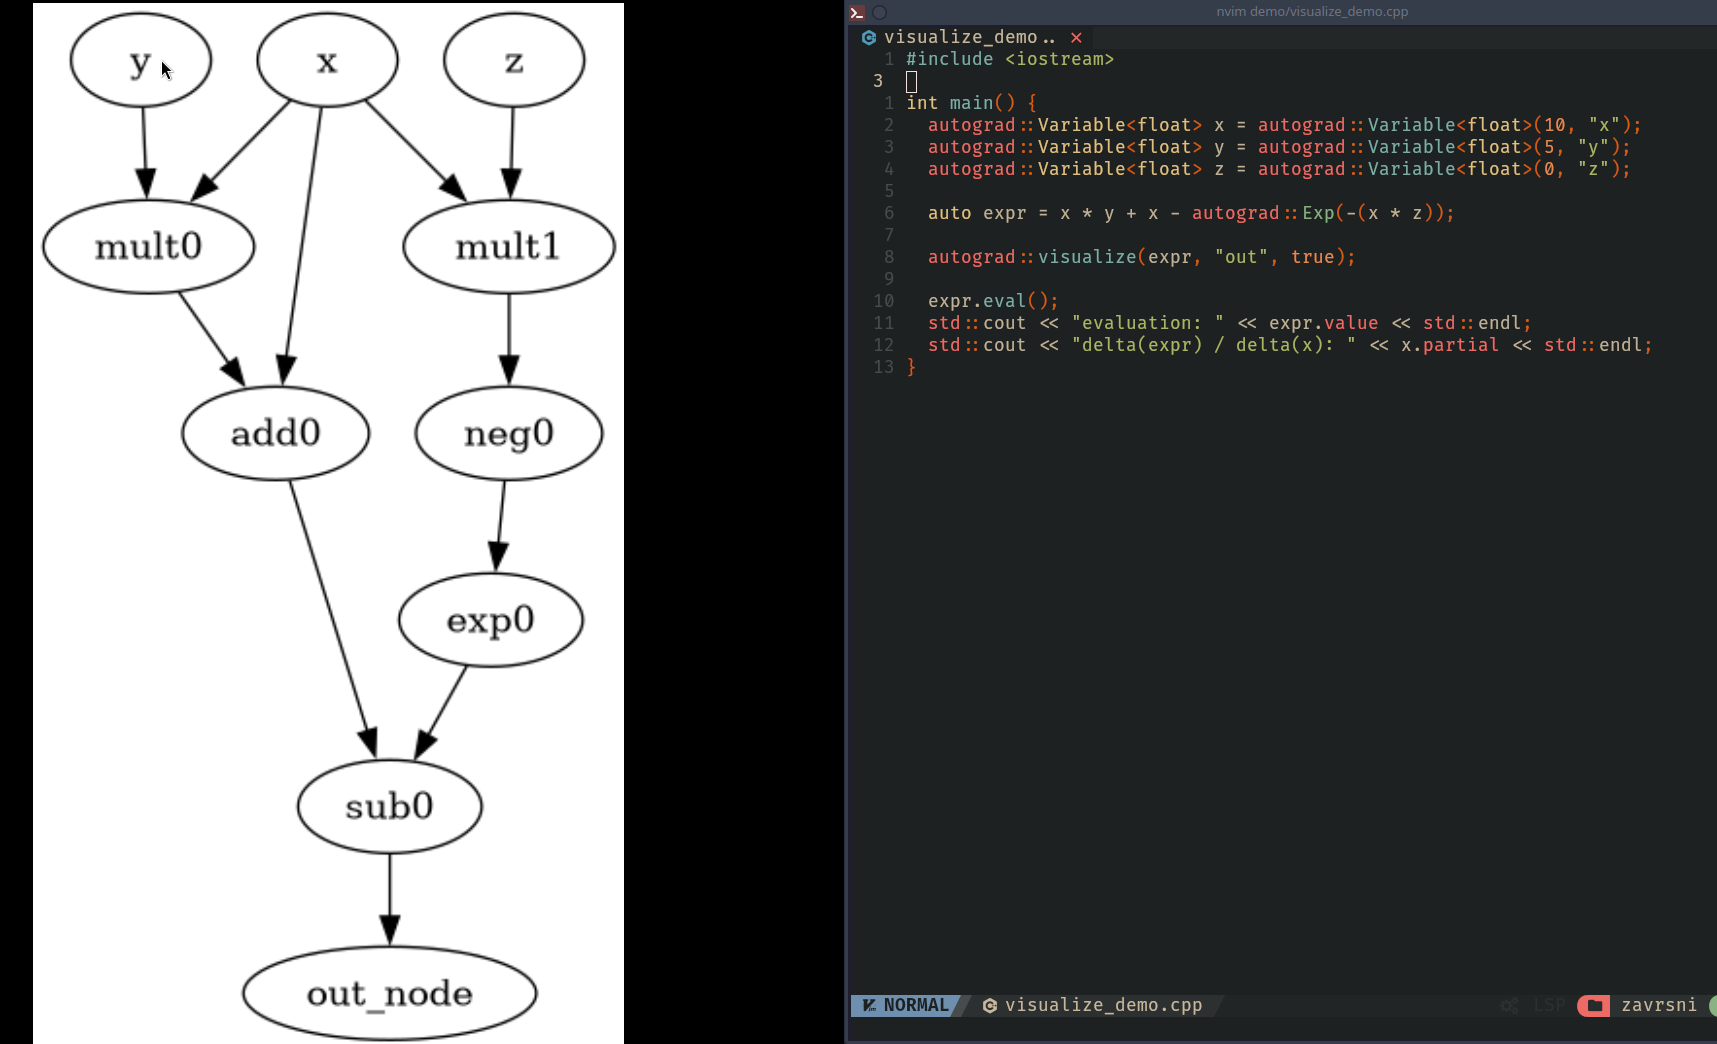
\includegraphics[width=0.7\linewidth]{../../pics/demo1.png}
  \caption{Primjer grafa funkcije: $f(x, y, z) = x * y + x - \exp(-x*z)$}
  \label{slk:prvaslika}
\end{figure}
\\
Općenito, za neku funkciju: $f\colon \mathbb{R}^n \rightarrow \mathbb{R}^m$ vrijedi da će njezin graf imati $n$ čvorova varijabli, odnosno $n$ izvora te $m$ izlaznih čvorova, tj. $m$ ponora. Dodatno možemo pojednostaviti njezin graf ako funkciju zamislimo kao $f\colon \mathbb{V}^n \rightarrow \mathbb{V}^m$ te zatim predstavimo sve varijable kao vektore. Ta ideja će nam uvelike pojednostaviti samu implementaciju autograd programa jer će apstrahirati prijelaz s univarijatnih na multivarijatne funkcije.
\\
TODO: nastavi o različitim metodama autograda i reprezentacijama objekata...

\section{OpenCL i C++}
Referenciramo se na sliku \ref{slk:prvaslika} u sredini rečenice, zatim prije zareza \ref{slk:prvaslika}, te zatim na kraju rečenice \ref{slk:prvaslika}.
Upravo smo testirali radi li naredba \verb|\ref| ispravno u slučaju kada nakon nje slijedi točka.
\blindtext

Sada slijedi jedna jednadžba:
\begin{equation}
  \label{jed:prvajednadzba}
  \int_{-\infty}^{+\infty}f(t)\,dt=F(\omega)
\end{equation}
Jednadžba \eqref{jed:prvajednadzba} je moja prva jednadžba koja defnira par $f(t)\ufrek F(\omega)$ ili $F(\omega)\uvrem f(t)$.


%-------------------------------------------------------------------------------
\chapter{Glavni dio}
\label{pog:glavni_dio}

Ovdje ide glavni dio rada... TODO
\blindtext

%-------------------------------------------------------------------------------
\chapter{Rezultati i rasprava}
\label{pog:rezultati_i_rasprava}

Rezultati su jako dobri... TODO: napisi ih
\blindtext


%--- ZAKLJUČAK / CONCLUSION ----------------------------------------------------
\chapter{Zaključak}
\label{pog:zakljucak}

Zaključno, TODO...
\blindtext


%--- LITERATURA / REFERENCES ---------------------------------------------------

% Literatura se automatski generira iz zadane .bib datoteke / References are automatically generated from the supplied .bib file
% Upiši ime BibTeX datoteke bez .bib nastavka / Enter the name of the BibTeX file without .bib extension
\bibliography{literatura}



%--- SAŽETAK / ABSTRACT --------------------------------------------------------

% Sažetak na hrvatskom
\begin{sazetak}
  TODO: Unesite sažetak na hrvatskom.
  \blindtext
\end{sazetak}

\begin{kljucnerijeci}
  TODO: ključčne riječi
  prva ključna riječ; druga ključna riječ; treća ključna riječ
\end{kljucnerijeci}


% Abstract in English
\begin{abstract}
  This is the abstract in english. TODO: write a proper one...
  \blindtext
\end{abstract}

\begin{keywords}
  the first keyword; the second keyword; the third keyword
\end{keywords}


%--- PRIVITCI / APPENDIX -------------------------------------------------------

% Sva poglavlja koja slijede će biti označena slovom i riječi privitak / All following chapters will be denoted with an appendix and a letter
\backmatter

\chapter{The Code}

Ovdje ide kod... TODO: dodaj ga


\end{document}
